\documentclass[12pt]{report}

\usepackage{amssymb, fullpage, amsmath,mathdots}
\usepackage{graphicx}

\newtheorem{problem}{Problem}

\newenvironment{solution}[1][\it{Solution}]{\textbf{#1. } }{$\square$}

\graphicspath{ {./} }

\pagestyle{empty}

\def\Z{{\mathbb Z}}
\def\Q{{\mathbb Q}}
\def\C{{\mathbb C}}
\def\R{{\mathbb R}}
\def\N{{\mathbb N}}

\begin{document}

\large

\begin{center}
 Math 584 Homework 3\\
 Due Wednesday Oct 18\\
 By Marvyn Bailly\\
\end{center}

\normalsize

\hrule

%---------------%
%---Problem 1---%
%---------------%

%--status--$

\begin{problem}
    6.1
\end{problem}

\begin{solution}
    \noindent
    
    Let $P$ be an orthogonal projector. We wish to show that $I - 2P$ is unitary. Since $P$ is a projector we know that $P^2 = P$, and since it is an orthogonal projector we know that $P = P^*$. Now observe that 
    \begin{align*}
        (I - 2P)^*(I - 2P) &= (I - 2P^*)(I - 2P)\\
        &= (I - 2P)(I - 2P)\\
        &= I - I2P - I2P + 4P^2\\
        &= I - 4P + 4P^2\\
        &= I - 4P + 4P\\
        &= I
    \end{align*}
    Thus we have shown that the columns of $I$ are orthogonal.

    \begin{center}
        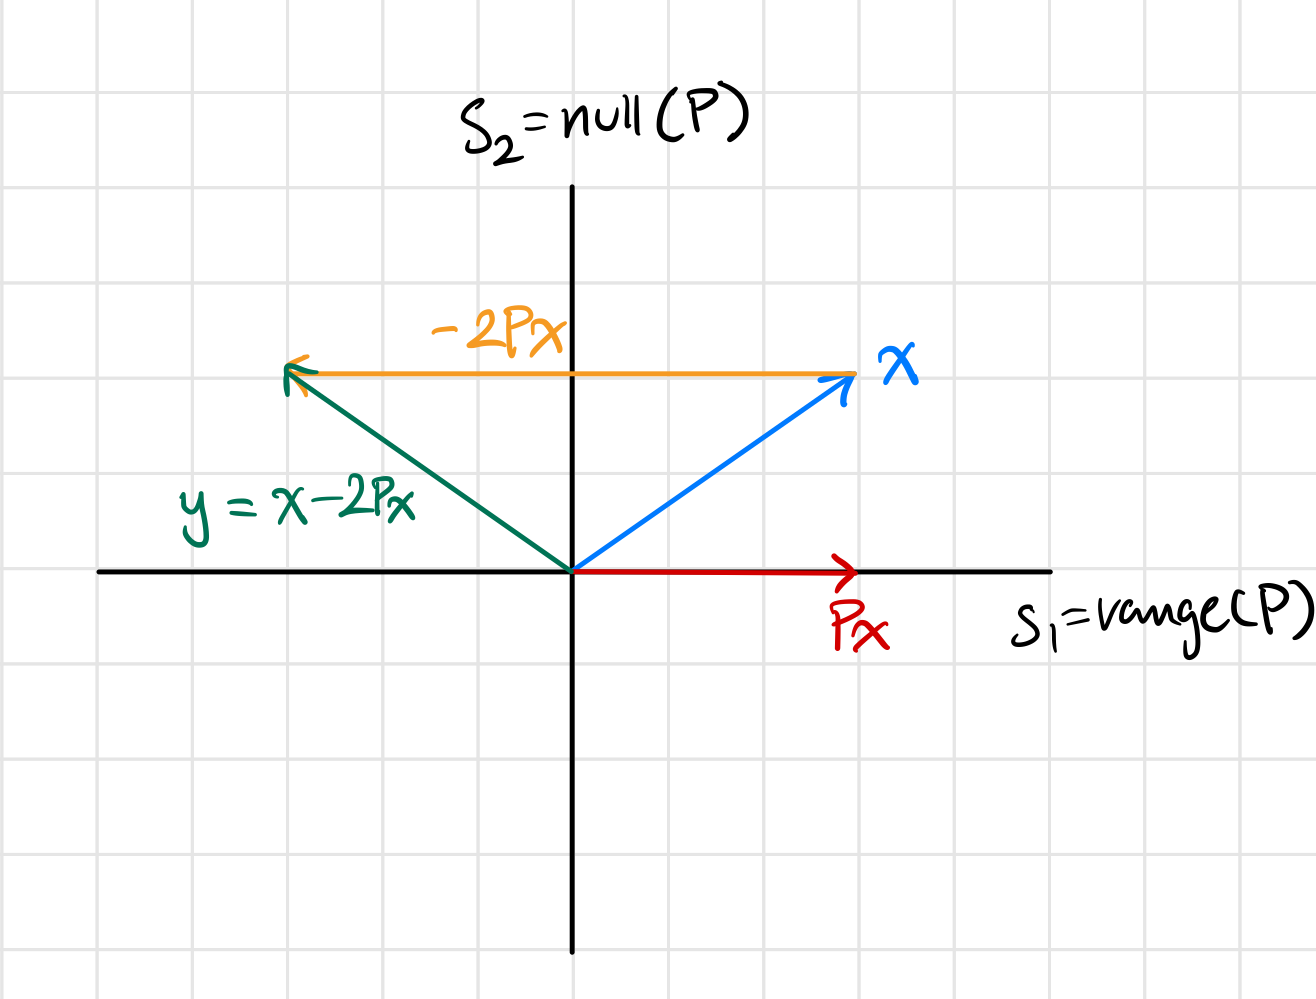
\includegraphics[width=.4\textwidth]{fig.png}
    \end{center}

    Looking at the image kindly made by Rohin, we visual how $(I - 2P)x = x - 2Px$ and see that it mirrors over the null space of $S_2$. We can visually see that the length $x$ remains the same under the transformation. And since the applying the transformation will move the vector back in the opposite direction, $x - 2Px$ is unitary.  
\end{solution}

%----------------------------------------------------------------------------------------------------%
%\vskip 20pt
\newpage

%---------------%
%---Problem 2---%
%---------------%

%--status--$

\begin{problem}
    6.2
\end{problem}

\begin{solution}
    \noindent
    Let $E$ be the $m\times m$ matrix that extracts "even part" of an vector:
    \[ 
        Ex = \frac{x + Fx}{2}
    \]
    where $F$ is the $m \times m$ matrix that flips $(x_1, \cdots, x_m)^*$ to $(x_m, \cdots, x_1)^*$. To check if $E$ is an projector observe that $Ex$ can be rewritten as,
    \[ 
        Ex = \frac{x + Fx}{2} = \frac{1}{2}\left(I + F\right)x.
    \]
    with this simplification see that,
    \begin{align*}
        (E)^2 &= \left( \frac{1}{2}(I + F)\right)^2\\
        &= \frac{1}{4} \left(I + F\right)^2\\
        &= \frac{1}{4} \left(2F + F^2 + 2I\right)\\
        &= \frac{1}{4} \left(2F + I + I\right)\\
        &= \frac{1}{2} \left(F + I\right)\\
        &= E
    \end{align*}
    which implies that $E^2 = E$ verifying that $E$ is a projector. Note that $F^2$ flips $(x_1, \cdots, x_m)^*$ to $(x_m, \cdots, x_1)^*$ and then flip it back, thus $F^2 = I$. Next let's check to see if $E$ is an orthogonal projector by checking if $E^* = E$. Computing this we see that,
    \[E^* = \frac{1}{2}(I + F)^* = \frac{1}{2}(F^* +I) \]
    and thus $E$ is orthogonal if $F$ is symmetric, so let's compute the entries of $F$. We know that $F$ flips $(x_1, \cdots, x_m)^*$ to $(x_m, \cdots, x_1)^*$ and thus $F$ most be of the form,
    \[
        F = \begin{pmatrix}
             0&\cdots&0&0&1\\
             0&\cdots&0&1&0\\
             0&\cdots&1&0&0\\
             &\iddots&\vdots&\vdots&\vdots\\
             1&\cdots&0&0&0
        \end{pmatrix}
    \] 
    This matrix is indeed symmetric and thus $E$ is indeed an orthogonal projector. To find the entries of $E$, notice that, 
    \[ E = (I + F) = \frac{1}{2}\begin{pmatrix} 1 & 0 & 0 & \cdots & 0\\ 0 & 1 & 0  & \cdots & 0 \\ 0 & 0 & 1 & \cdots & 0 \\ \vdots & \vdots & \vdots & \ddots \\ 0 & 0 & 0 & \cdots & 1\end{pmatrix} + \begin{pmatrix}
        0&\cdots&0&0&1\\
        0&\cdots&0&1&0\\
        0&\cdots&1&0&0\\
        &\iddots&\vdots&\vdots&\vdots\\
        1&\cdots&0&0&0
   \end{pmatrix}
    \]
   Thus $E$ is given by
   \[
        E = \frac{1}{2}\begin{cases}
            \begin{pmatrix}
                1&0&0&\cdots&0&\cdots&0&0&1\\
                0&1&0&\cdots&0&\cdots&0&1&0\\
                0&0&\ddots&&\vdots&&\iddots&0&0\\
                \vdots&\vdots&&1&0&1&&\vdots&\vdots\\
                0&0&\cdots&0&2&0&\cdots&0&0\\
                \vdots&\vdots&&1&0&1&&\vdots&\vdots\\
                0&0&\iddots&&\vdots&&\ddots&0&0\\
                0&1&0&\cdots&0&\cdots&0&1&0\\
                1&0&0&\cdots&0&\cdots&0&0&1\\
            \end{pmatrix}, & \text{when $m$ is odd}\\
            \\
            \begin{pmatrix}
                1&0&0&\cdots&0&0&\cdots&0&0&1\\
                0&1&0&\cdots&0&0&\cdots&0&1&0\\
                0&0&1&&\vdots&\vdots&&1&0&0\\
                \vdots&\vdots&&\ddots&0&0&\iddots&&\vdots&\vdots\\
                0&0&\cdots&0&1&1&0&\cdots&0&0\\
                0&0&\cdots&0&1&1&0&\cdots&0&0\\
                \vdots&\vdots&&\iddots&0&0&\ddots&&\vdots&\vdots\\
                0&0&1&&\vdots&\vdots&&1&0&0\\
                0&1&0&\cdots&0&0&\cdots&0&1&0\\
                1&0&0&\cdots&0&0&\cdots&0&0&1\\
            \end{pmatrix}, &\text{when $m$ is even.}
        \end{cases}
   \]
\end{solution}

%----------------------------------------------------------------------------------------------------%
%\vskip 20pt
\newpage

%---------------%
%---Problem 3---%
%---------------%

%--status--$

\begin{problem}
    6.4
\end{problem}

\begin{solution}


    \noindent
    Consider the matrices 
    \[
        A = \begin{pmatrix}
            1&0\\0&1\\1&0
        \end{pmatrix}, ~~~~~ B = \begin{pmatrix}
            1&2\\0&1\\1&0
        \end{pmatrix}.
    \]
    
    \begin{enumerate}
        \item [{\bf a}] We wish to find an orthogonal projector $P_A$ onto range($A$). Let's use the fact that $P_A = A(A^*A)^{-1}A^*$ to compute the orthogonal projector to get,
        \begin{align*}
            P_A &= A(A^*A)^{-1}A^*\\
            &= \begin{pmatrix}
                1&0\\0&1\\1&0
            \end{pmatrix}\left( \begin{pmatrix}
                1&0\\0&1\\1&0
            \end{pmatrix}^* \begin{pmatrix}
                1&0\\0&1\\1&0
            \end{pmatrix}\right)^{-1}\begin{pmatrix}
                1&0\\0&1\\1&0
            \end{pmatrix}^*\\
            &= \begin{pmatrix}
                1&0\\0&1\\1&0
            \end{pmatrix}\left( \begin{pmatrix}1&0&1\\ 0&1&0\end{pmatrix} \begin{pmatrix}
                1&0\\0&1\\1&0
            \end{pmatrix}\right)^{-1}\begin{pmatrix}1&0&1\\ 0&1&0\end{pmatrix}\\
            &= \begin{pmatrix}
                1&0\\0&1\\1&0
            \end{pmatrix}\begin{pmatrix}\frac{1}{2}&0\\ 0&1\end{pmatrix}\begin{pmatrix}1&0&1\\ 0&1&0\end{pmatrix}\\
            &= \begin{pmatrix}\frac{1}{2}&0&\frac{1}{2}\\ 0&1&0\\ \frac{1}{2}&0&\frac{1}{2}\end{pmatrix}
        \end{align*}\\
        Then we can find the image of the vector $(1,2,3)^*$ under $P_A$ by computing,
        \[
            P_A(1,2,3)^* = \begin{pmatrix}
                1/2&0&1/2\\
                0&1&0\\
                1/2&0&1/2
            \end{pmatrix} \begin{pmatrix}
                1\\2\\3
            \end{pmatrix} = \begin{pmatrix}
                2\\2\\2
            \end{pmatrix}
        \] 

        \item [{\bf b}] Next we wish to find an orthogonal projector $P_B$ onto the range($B$). Let's use the fact that $P_B = B(B^*B)^{-1}B^*$ to compute the orthogonal projector to get,
        \begin{align*}
            P_B &= \begin{pmatrix}
                1&2\\0&1\\1&0
            \end{pmatrix} \left( \begin{pmatrix}1&0&1\\ 2&1&0\end{pmatrix} \begin{pmatrix}
                1&2\\0&1\\1&0
            \end{pmatrix} \right)^{-1} \begin{pmatrix}1&0&1\\ 2&1&0\end{pmatrix}\\
            &= \begin{pmatrix}
                1&2\\0&1\\1&0
            \end{pmatrix} \begin{pmatrix}2&2\\ 2&5\end{pmatrix}^{-1}\begin{pmatrix}1&0&1\\ 2&1&0\end{pmatrix}\\
            &= \begin{pmatrix}
                1&2\\0&1\\1&0
            \end{pmatrix}\begin{pmatrix}\frac{5}{6}&-\frac{1}{3}\\ -\frac{1}{3}&\frac{1}{3}\end{pmatrix}\begin{pmatrix}1&0&1\\ 2&1&0\end{pmatrix}\\
            &= \begin{pmatrix}\frac{5}{6}&\frac{1}{3}&\frac{1}{6}\\ \frac{1}{3}&\frac{1}{3}&-\frac{1}{3}\\ \frac{1}{6}&-\frac{1}{3}&\frac{5}{6}\end{pmatrix}
        \end{align*}
        Then we can find the image of the vector $(1,2,3)^*$ under $P_B$ by computing,
        \[
            P_B(1,2,3)^* = \begin{pmatrix}\frac{5}{6}&\frac{1}{3}&\frac{1}{6}\\ \frac{1}{3}&\frac{1}{3}&-\frac{1}{3}\\ \frac{1}{6}&-\frac{1}{3}&\frac{5}{6}\end{pmatrix} \begin{pmatrix}
                1\\2\\3
            \end{pmatrix} = \begin{pmatrix}2\\0\\2\end{pmatrix}.
        \]
    \end{enumerate}
\end{solution}

%----------------------------------------------------------------------------------------------------%
%\vskip 20pt
\newpage

%---------------%
%---Problem X---%
%---------------%

%--status--$

\begin{problem}
    7.1
\end{problem}

\begin{solution}
    \noindent
    Consider the matrices,
    \[
        A = \begin{pmatrix}
            1&0\\0&1\\1&0
        \end{pmatrix}, ~~~~~ B = \begin{pmatrix}
            1&2\\0&1\\1&0
        \end{pmatrix}.
    \]

    \begin{enumerate}
        \item [{\bf a}] Consider matrix $A$. First let's find the reduced QR factorization $A = \hat{Q}\hat{R}$ by using the Gram Schmitt algorithm where $a_1 = (1,0,1)^*$ and $a_2 = (0,1,0)^*$. First we can find $q_1$ by computing,
        \[
            q_1 = \frac{a_1}{\|a_1\|} = \begin{pmatrix}
                1/\sqrt{2}\\0\\1/\sqrt{2}
            \end{pmatrix}
        \]
        which also gives that \[r_{11} = \sqrt{2}\].
        Next we can compute,
        \begin{align*}
            \tilde{q_2} &= a_2 - (q_1^*a_2)q_1\\
            &= \begin{pmatrix}
                0\\1\\0
            \end{pmatrix} - \left( (1/\sqrt{2}, 0, 1/\sqrt{2}) \begin{pmatrix}
                0\\1\\0
            \end{pmatrix}\right)\begin{pmatrix}
                1/\sqrt{2}\\0\\1/\sqrt{2}
            \end{pmatrix}\\
            &= \begin{pmatrix}
                0\\1\\0
            \end{pmatrix} - \left( 0 \right)\begin{pmatrix}
                1/\sqrt{2}\\0\\1/\sqrt{2}\\
            \end{pmatrix}\\
            &= \begin{pmatrix}
                0\\1\\0
            \end{pmatrix}
        \end{align*}
        so $\tilde{q_2} = \begin{pmatrix}
            0\\1\\0
        \end{pmatrix}$ which means that,
        \[ q_2 = \frac{\tilde{g_2}}{\sqrt{1}} = \begin{pmatrix}
            0\\1\\0
        \end{pmatrix}.\]
        Along the way we also get that $r_{12} = 0$ and $r_{22} = 1$. Therefore we have that the reduced QR factorization of $A$ is given by,
        \[A = \hat{Q}\hat{R} = \begin{pmatrix}
            1/\sqrt{2} & 0\\
            0 & 1\\
            1/\sqrt{2} & 0
        \end{pmatrix} \begin{pmatrix}
            \sqrt{2} & 0\\
            0 & 1
        \end{pmatrix}.\] 
        To find the full QR factorization we need to compute $Q$ and $R$. We can easily find $R$ to be,
        \[
            R = \begin{pmatrix}
                \sqrt{2}&0\\ 0&1\\ 0&0 
            \end{pmatrix}.
        \]
        Next we need to find a column that is orthonormal to the columns of $A$. To find a vector that is orthogonal, consider
        \[
            \begin{pmatrix}1/\sqrt{2}&0&1/\sqrt{2}\\0&1&0\end{pmatrix}\begin{pmatrix}a\\b\\c\end{pmatrix} = \begin{pmatrix}
                0\\0
            \end{pmatrix}
        \]
        which gives that $a=-c$ and $b=0$. And since the vector must also be orthonormal, it is also restricted to be $\sqrt{a^2 + b^2 + c^2} = \sqrt{a^2 + a^2} = \sqrt{2a^2}$ which means that $a = \frac{1}{\sqrt{2}}$. Thus we have found the QR factorization to be,
        \[ 
            A = QR = \begin{pmatrix}
                1/\sqrt{2}&0&1/\sqrt{2}\\
                0&1&0\\
                1/\sqrt{2}&0&-1/\sqrt{2}\\
            \end{pmatrix}\begin{pmatrix}
                \sqrt{2}&0\\ 0&1\\ 0&0 
            \end{pmatrix}.
        \]

        \item [{\bf b}] Consider matrix $B$. First let's find the reduced QR factorization $B = \hat{Q}\hat{R}$ by using the Gram Schmitt algorithm where $b_1 = (1,0,1)^*$ and $b_2 = (2,1,0)^*$. First we can find $q_1$ by computing,
        \[ 
            q_1 = \frac{b_1}{\|b_1\|} = (1/\sqrt{2}, 0, 1\sqrt{2})^*
        \]
        and this also gives us,
        \[
            r_{11} = \sqrt{2}.
        \]
        Next we can compute,
        \begin{align*}
            \tilde{q_2} &= b_2 - (q_1^*b_2)q_1\\
            &= \begin{pmatrix}
                2\\1\\0
            \end{pmatrix} - \left[ \left(1/\sqrt{2}, 0 ,1/\sqrt{2} \right) \begin{pmatrix} 2\\1\\0 \end{pmatrix}\right]\begin{pmatrix}
                1/\sqrt{2}\\
                0\\
                1/\sqrt{2}
            \end{pmatrix}\\
            &= \begin{pmatrix}
                2\\1\\0
            \end{pmatrix} - \frac{2}{\sqrt{2}}\begin{pmatrix}
                1/\sqrt{2}\\
                0\\
                1/\sqrt{2}
            \end{pmatrix}\\
            &= \begin{pmatrix}
                2\\1\\0
            \end{pmatrix} - \begin{pmatrix}
                1\\
                0\\
                1
            \end{pmatrix}
        \end{align*}
        Thus $\tilde{q_2} = (1,1,-1)^*$ and we get,
        \[
            q_2 = \frac{\tilde{q_2}}{\|\tilde{q_2}\|} = \begin{pmatrix}
                1/\sqrt{3}\\ 1/\sqrt{3}\\ -1/\sqrt{3}
            \end{pmatrix}
        \]
        We also gained along the way that $r_{12} = q_1^*b_2 = \frac{2}{\sqrt{2}}$ and $r_{22} = \sqrt{3}$. Thus we have calculated the reduced QR factorization of $B$ to be,
        \[
            B = \tilde{Q}\tilde{R} = \begin{pmatrix}
                1/ \sqrt{2} & 1/ \sqrt{3}\\
                0 & 1/\sqrt{3}\\
                1/\sqrt{2} & -1/\sqrt{3}\\
            \end{pmatrix}\begin{pmatrix}
                \sqrt{2} & 2/\sqrt{2}\\
                0 & \sqrt{3}
            \end{pmatrix}.
        \]
        To find the full QR factorization, we need to compute $Q$ and $R$. We can easily find $R$ to be,
        \[
            R = \begin{pmatrix}
                \sqrt{2} & 2/\sqrt{2}\\
                0 & \sqrt{3}\\
                0&0
            \end{pmatrix}.
        \]
        Next we need to find a column that is orthonormal to the columns of $B$. To find a vector that is orthogonal consider, 
        \[
            \begin{pmatrix}
                1/\sqrt{2} & 0 & 1/\sqrt{2}\\
                1/\sqrt{3} & 1/\sqrt{3} & -1/\sqrt{3}
            \end{pmatrix}\begin{pmatrix}
                a\\b\\c
            \end{pmatrix} = \begin{pmatrix}
                0\\0
            \end{pmatrix}
        \]
        which tells us that $a = -c$ and $b =-2a = 2c$. To restrict the column to be orthonormal we must have $\sqrt{a^2 + b^2 + c^2} = \sqrt{a^2 + (-2a)^2 + (-2a)^2} = \sqrt{6a^2} = \sqrt{6}a=1$ Thus we have that $a = 1 / \sqrt{6}$ so $b = -2 / \sqrt{6}$ and $c = - 1/\sqrt{6}$. Which gives us the full QR factorization to be,
        \[
            B = QR = \begin{pmatrix}
                1/ \sqrt{2} & 1/ \sqrt{3} & 1/ \sqrt{6}\\
                0 & 1/\sqrt{3} & -2 / \sqrt{6}\\
                1/\sqrt{2} & -1/\sqrt{3} & - 1/\sqrt{6}\\
            \end{pmatrix}\begin{pmatrix}
                \sqrt{2} & 2/\sqrt{2}\\
                0 & \sqrt{3}\\
                0 & 0
            \end{pmatrix}.
        \]
    \end{enumerate}
\end{solution}

%----------------------------------------------------------------------------------------------------%
%\vskip 20pt
\newpage

%---------------%
%---Problem 5---%
%---------------%

%--status--$

\begin{problem}
    8.1
\end{problem}

\begin{solution}
    \noindent
    Consider the Modified Gram-Schmidt algorithm given by,
    \begin{center}
        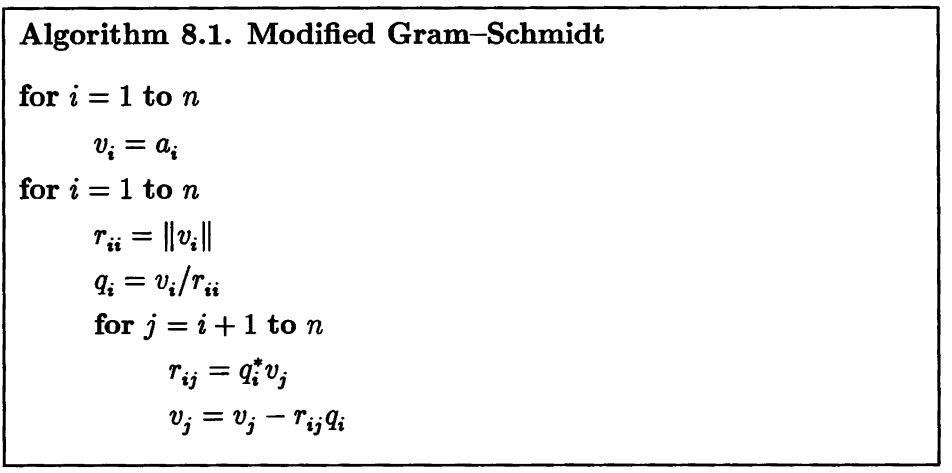
\includegraphics[width=.4\textwidth]{alg8.1.JPG}.
    \end{center} 
    We will count the number of operations by type. I'll begin with addition. From the outer loop we have $m-1$ additions from the $r_ii = \| v_i \|$ term and from the inner loop, we have $m-1$ additions from the $r_{ij} = q_i^*v_j$ term. Thus there are,
    \begin{align*}
        \sum_{i=1}^n (m-1)(n-i) + \sum_{i=1}^n(m-1) &= \frac{1}{2}(m-1)n(n - 1) + (m-1)(n)\\
        &= \frac{(m-1)n(n+1)}{2}.
    \end{align*} 
    Next let's count the number of substractions. From the inner loop, there are $m$ substracts from the $v_j = v_j - r_{ij}q_i$ term. Thus there are,
    \[
        \sum_{i=1}^n m(n-1) = \frac{mn(n-1)}{2}.
    \]
    Next let's count the multiplications. From the inner loop we have $m$ multiplications from the $r_ii = \| v_i \|$ term, and the inner loop we have, both terms give $m$ multiplications. Thus there are,
    \[ 
        \sum_{i=1}^n 2m(n-1) + \sum_{i=1}^nm = mn(n-1) + mn = mn^2.
    \]
    And finally let's count the number of division. From the outer loop we have, $m$ divisions from the $q_i = v_i/r_{ii}$ term. Thus there are $mn$ divisions. Adding all these up we get the total flops to be,
    \begin{align*}
        \frac{(m-1)n(n+1)}{2} + \frac{mn(n-1)}{2} + mn^2 + mn &= \frac{1}{2 n ((2 m - 1) n - 1)} + mn^2 + mn\\
    \end{align*}
\end{solution}

%----------------------------------------------------------------------------------------------------%
%\vskip 20pt
\newpage

%---------------%
%---Problem X---%
%---------------%

%--status--$

\begin{problem}
    11.3
\end{problem}

\begin{solution}
    
    \noindent
    I created the MatLab code, 
    \begin{verbatim}
        function q11()
        format long;
        m = 50; n = 12;
        t = linspace(0,1,m);
        
        A = fliplr(vander(t));
        A = A(:,1:12);
        b = cos(4*t)';
        
        %Method A - Normal Equation%
        R = chol(A'*A);
        xa = R\(R'\(A'*b));
        
        %Method D - QR factorization%
        [Q, R] = qr(A);
        xd = R\(Q'*b);
        
        %Method E - A\b%
        xe = A\b;
        
        %Method F - SVD factorization%
        [U, S, V] = svd(A,0);
        xf = V*(S\(U'*b));
        
        x = [xa, xd, xe, xf]
        end
    \end{verbatim}
    \pagebreak
    to print the least square coefficients of the four methods. The code outputs,
    \begin{verbatim}
Method A             Method D            Method E            Method F
 0.999999996787553   1.000000000996608   1.000000000996607   1.000000000996608
 0.000000350916732  -0.000000422743080  -0.000000422743364  -0.000000422743088
-8.000003028795119  -7.999981235685203  -7.999981235676154  -7.999981235684746
-0.000077893877909  -0.000318763231287  -0.000318763346323  -0.000318763237547
 10.668084035612900  10.669430795858052  10.669430796641096  10.669430795900578
-0.009615585352545  -0.013820287698367  -0.013820290914619  -0.013820287867134
-5.654480747960067  -5.647075628404193  -5.647075619959385  -5.647075627982760
-0.068885958631546  -0.075316022079922  -0.075316036589419  -0.075316022763597
 1.693354534665567   1.693606960559036   1.693606976803618   1.693606961280185
 0.001461547101732   0.006032111063859   0.006032099645104   0.006032110585745
-0.370576739064076  -0.374241704456940  -0.374241699881279  -0.374241704275633
 0.087095866530693   0.088040576259675   0.088040575462356   0.088040576229626 
    \end{verbatim}
    which shows us that the results from methods D,E, and F are fairly consistent while method A is unstable. Observe,
    \begin{center}
        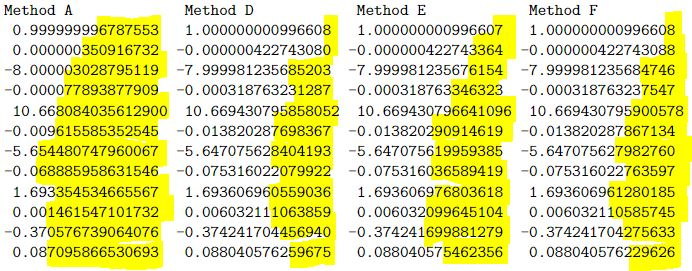
\includegraphics[width=.8\textwidth]{data.JPG}.
    \end{center} 
    where the highlighted lines show possible rounding error.This leads me to believe that the normal equations (method A) exhibit unstable behavior. 
\end{solution}

%----------------------------------------------------------------------------------------------------%
%\vskip 20pt
\newpage

%---------------%
%---Problem X---%
%---------------%

%--status--$

\begin{problem}
    Least Squares of Sport Teams
\end{problem}

\begin{solution}
    \noindent
    Consider the system of equations,
    \begin{align*}
        r_1 - r_2 = 4,\\
        r_3 - r_1 = 9,\\
        r_1 - r_4 = 6,\\
        r_3 - r_4 = 3,\\
        r_2 - r_4 = 7.
    \end{align*}
    \begin{enumerate}
        \item [{\bf a}]
        If we rewrite the system of equations as a matrix we get,
        \[ \begin{pmatrix}1&-1&0&0\\-1&0&1&0\\1&0&0&-1\\0&0&1&-1\\0&1&0&-1\end{pmatrix}\begin{pmatrix}
            r_1\\r_2\\r_3\\r_4
        \end{pmatrix} = \begin{pmatrix}
            4\\9\\6\\3\\7
        \end{pmatrix}.\]
        Now if we assume that $(r_1,r_2,r_3,r_4)^*$ is a solution for the system, observe $(r_1 +c ,r_2 + c,r_3 + c,r_4 + c)^*$ is also a solution for any constant $c$ since,
        \begin{align*}
            \begin{pmatrix}1&-1&0&0\\-1&0&1&0\\1&0&0&-1\\0&0&1&-1\\0&1&0&-1\end{pmatrix}\begin{pmatrix}
                r_1+c\\r_2+c\\r_3+c\\r_4+c
            \end{pmatrix} &= \begin{pmatrix}1\cdot \left(a+c\right)+\left(-1\right)\left(b+c\right)+0\cdot \left(c+c\right)+0\cdot \left(d+c\right)\\ \left(-1\right)\left(a+c\right)+0\cdot \left(b+c\right)+1\cdot \left(c+c\right)+0\cdot \left(d+c\right)\\ 1\cdot \left(a+c\right)+0\cdot \left(b+c\right)+0\cdot \left(c+c\right)+\left(-1\right)\left(d+c\right)\\ 0\cdot \left(a+c\right)+0\cdot \left(b+c\right)+1\cdot \left(c+c\right)+\left(-1\right)\left(d+c\right)\\ 0\cdot \left(a+c\right)+1\cdot \left(b+c\right)+0\cdot \left(c+c\right)+\left(-1\right)\left(d+c\right)\end{pmatrix}\\ &= \begin{pmatrix}a-b\\ c-a\\ a-d\\ c-d\\ b-d\end{pmatrix}\\
            &=\begin{pmatrix}
                4\\9\\6\\3\\7
            \end{pmatrix}      
        \end{align*} 
        as desired. Thus we append a sixth equation $r_1 + r_2 + r_3 + r_4 = 20$ to make the solution unique where $20$ is the total number of ranking points. 

        \item [{\bf b}]
        Notice that by adding a sixth equation, our new system of equations in matrix form will be, 
        \[ 
            \begin{pmatrix}1&-1&0&0\\ \:-1&0&1&0\\ \:1&0&0&-1\\ \:0&0&1&-1\\ \:0&1&0&-1\\ \:1&1&1&1\end{pmatrix}\begin{pmatrix}a\\ \:\:\:b\\ \:\:\:c\\ \:\:\:d\end{pmatrix} = \begin{pmatrix}
                4\\9\\6\\3\\7\\20
            \end{pmatrix}.
        \]
        We can see that the sixth equation will be exactly satisfied by observing,
        \begin{align*}
            \begin{pmatrix}1&-1&0&0\\ \:-1&0&1&0\\ \:1&0&0&-1\\ \:0&0&1&-1\\ \:0&1&0&-1\\ \:1&1&1&1\end{pmatrix}\begin{pmatrix}a\\ \:\:\:b\\ \:\:\:c\\ \:\:\:d\end{pmatrix} &= \begin{pmatrix}1\cdot \:a+\left(-1\right)b+0\cdot \:c+0\cdot \:d\\ \left(-1\right)a+0\cdot \:b+1\cdot \:c+0\cdot \:d\\ 1\cdot \:a+0\cdot \:b+0\cdot \:c+\left(-1\right)d\\ 0\cdot \:a+0\cdot \:b+1\cdot \:c+\left(-1\right)d\\ 0\cdot \:a+1\cdot \:b+0\cdot \:c+\left(-1\right)d\\ 1\cdot \:a+1\cdot \:b+1\cdot \:c+1\cdot \:d\end{pmatrix}\\
            &= \begin{pmatrix}a-b\\ c-a\\ a-d\\ c-d\\ b-d\\ a+b+c+d\end{pmatrix}\\
            &= \begin{pmatrix}
                4\\9\\6\\3\\7\\20
            \end{pmatrix}
        \end{align*}
        and thus we see that we can set the total number of ranking points to any number and the system will satisfy it. 

        \item [{\bf c}]
        I created the Matlab code,
        \begin{verbatim}
            A = [1,-1,0,0;-1,0,1,0;1,0,0,-1;0,0,1,-1;0,1,0,-1;1,1,1,1];
            b = [4;9;6;3;7;20];
            [Q, R] = qr(A);
            results = R\(Q'*b)
        \end{verbatim}
        that outputs,
        \begin{verbatim}
            results =
                5.2500
                4.6250
                9.1250
                1.0000
        \end{verbatim}
        using QR factorization to solve the least squares problem we have been discussing. based of this result, we know $T_3$ is in the lead with $T_1$ in second and $T_2$ in third.
    \end{enumerate}
\end{solution}

%----------------------------------------------------------------------------------------------------%
%\vskip 20pt
%\newpage

\end{document}